% [H] means put the figure HERE, directly when you input this code.
\begin{figure}[H]
	\centering
	
% We use a figure width of 48.5% of the width of one line of text on 
% the page so there is some space between the images.
	\subfloat[Top-Left image sub-caption.]{
		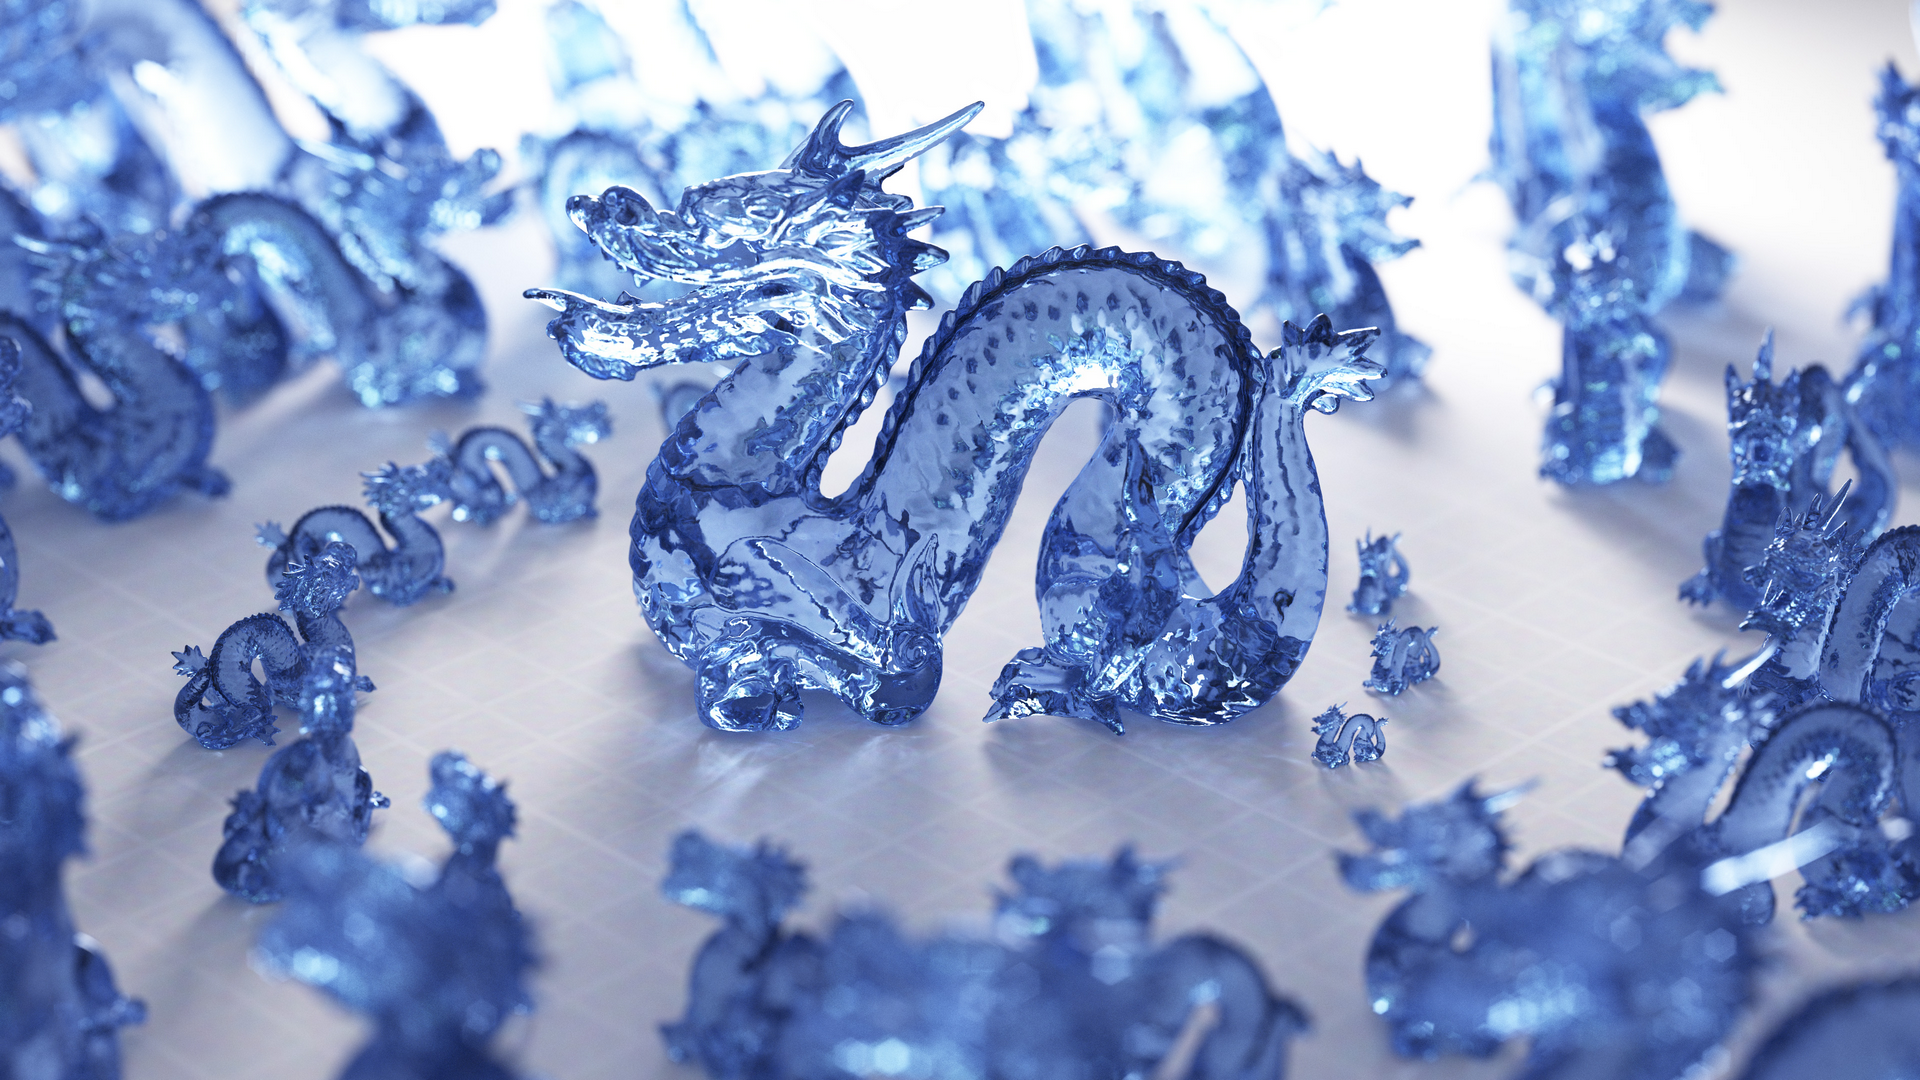
\includegraphics[width=0.485\linewidth]{./graphics/dragon.png}\label{fig:example_2x2_a}
	}~ % Use a tilde to add spacing for sub-figures that are displayed next to one another horizontally.
	\subfloat[Top-Right image sub-caption.]{
		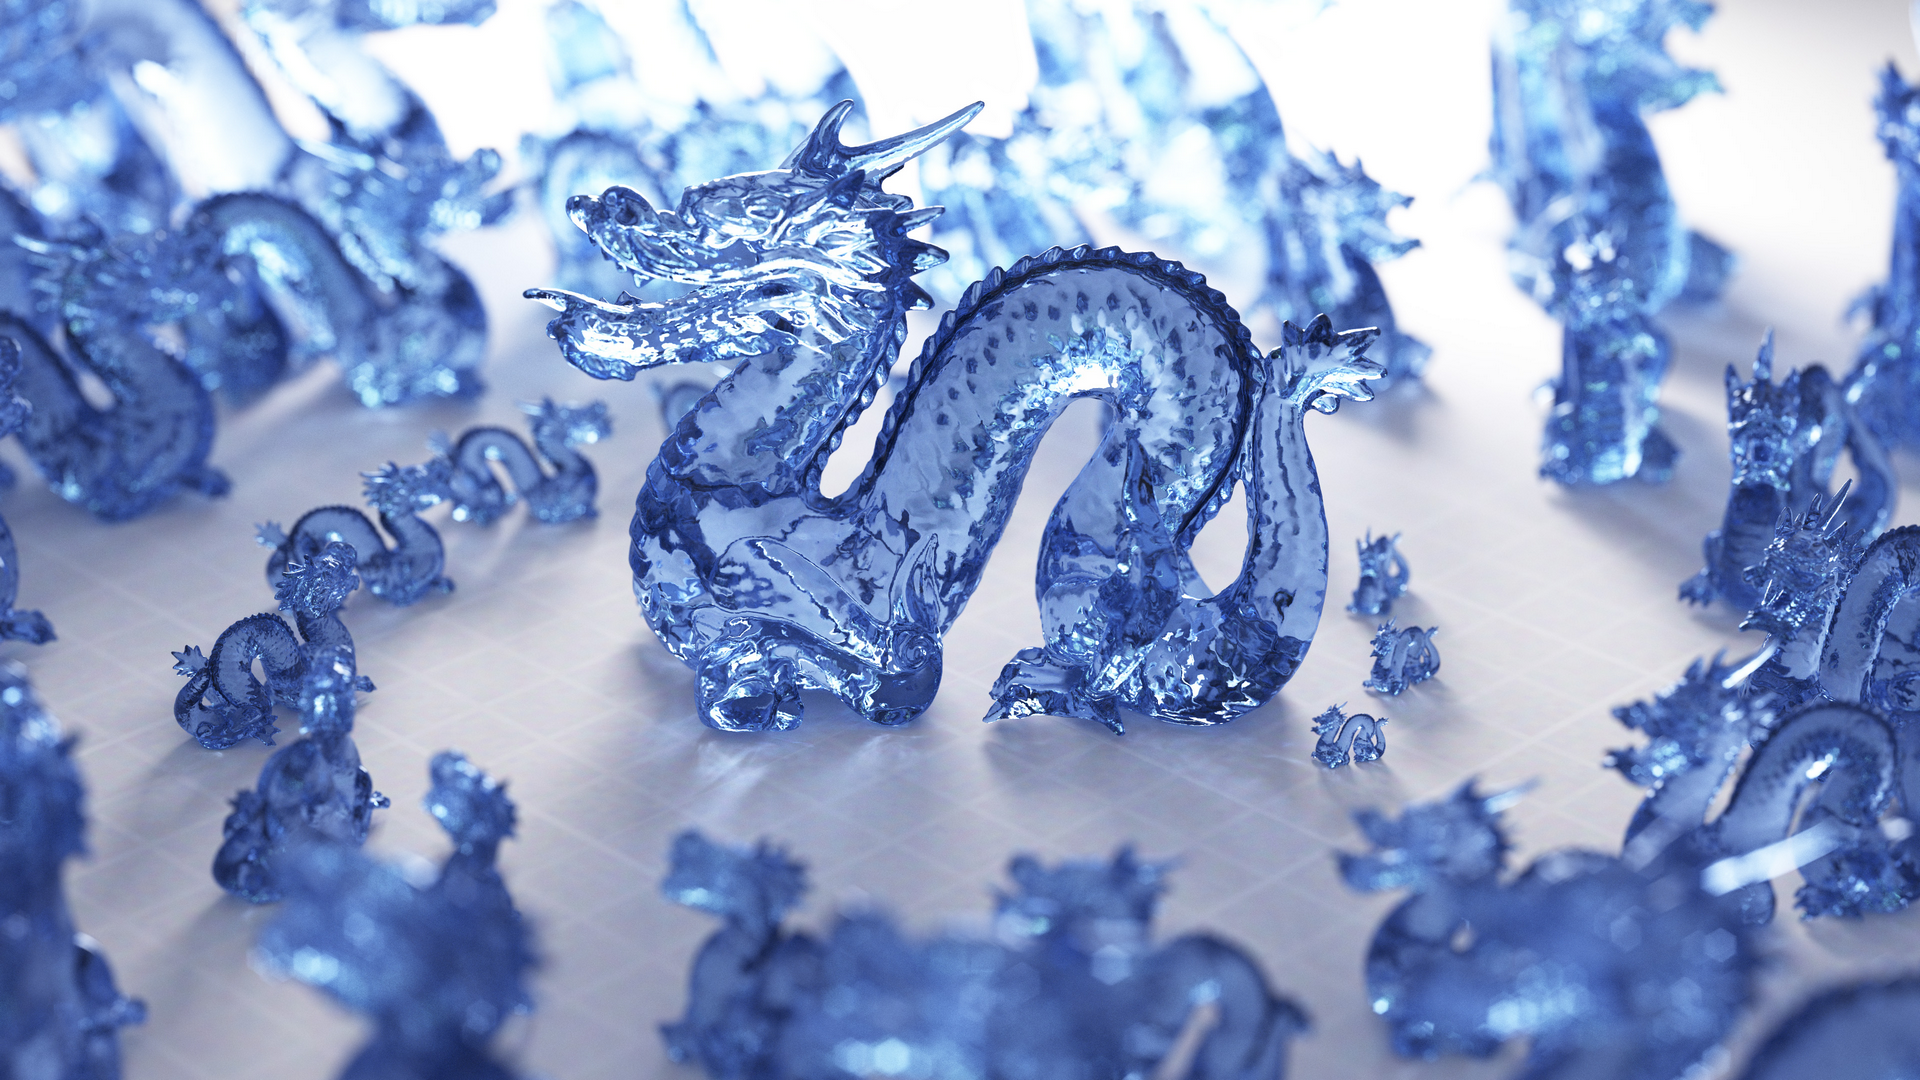
\includegraphics[width=0.485\linewidth]{./graphics/dragon.png}\label{fig:example_2x2_b}
	}\\ % New line before caption.
	\subfloat[Bottom-Left image sub-caption.]{
		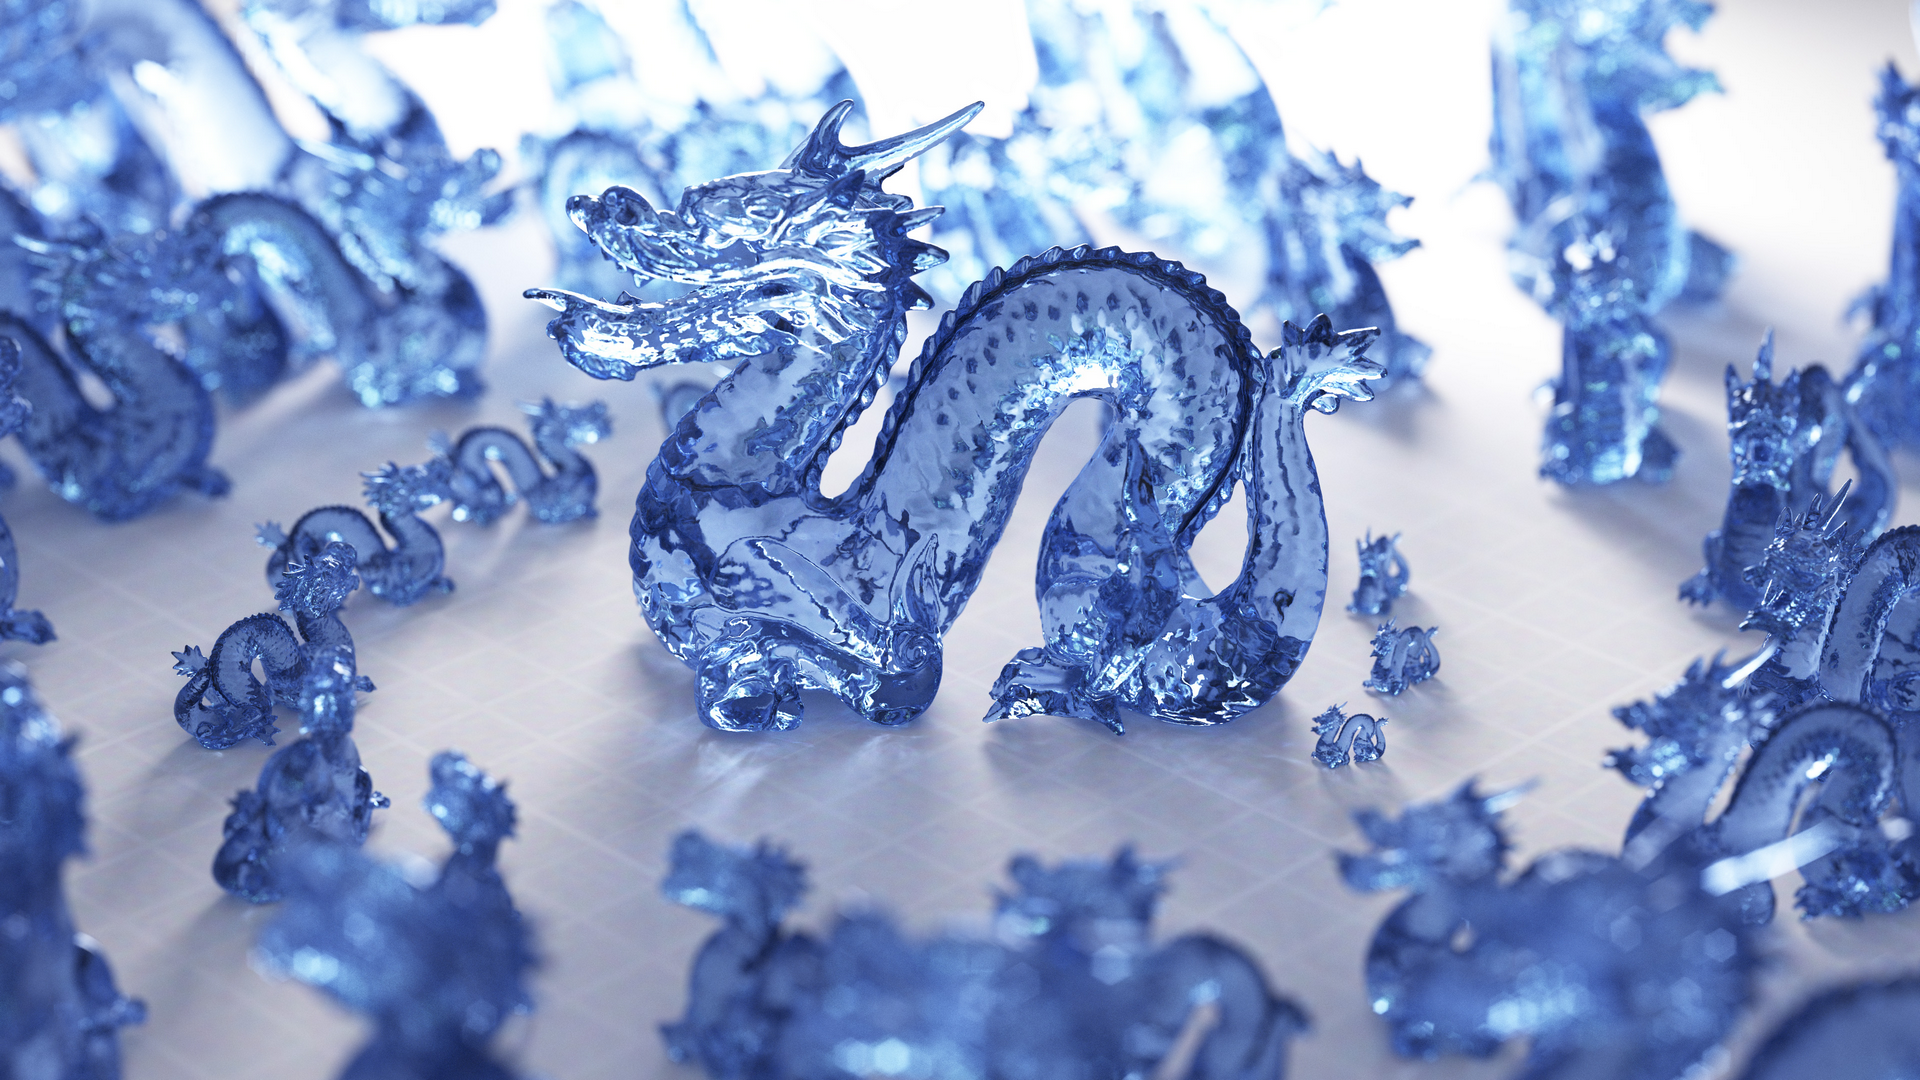
\includegraphics[width=0.485\linewidth]{./graphics/dragon.png}\label{fig:example_2x2_c}
	}~ % Use a tilde to add spacing for sub-figures that are displayed next to one another horizontally.
	\subfloat[Bottom-Right image sub-caption.]{
		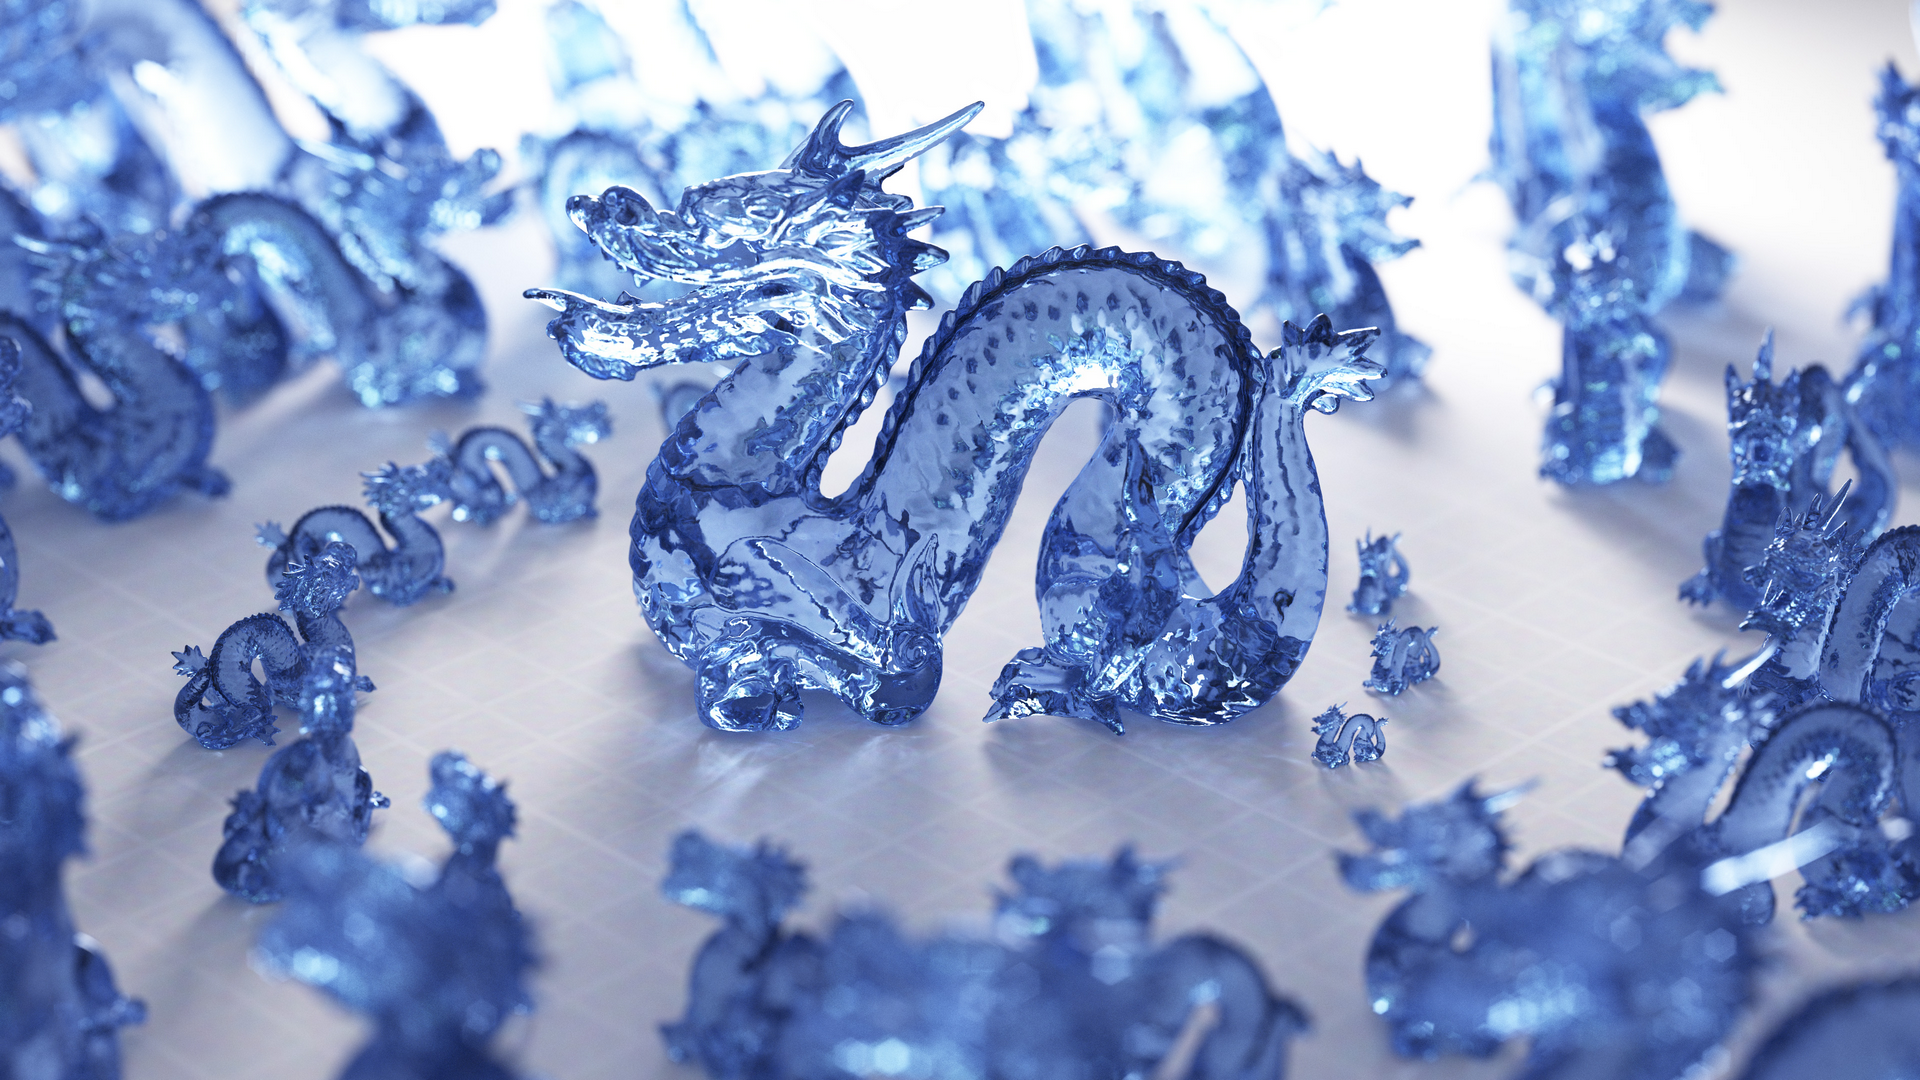
\includegraphics[width=0.485\linewidth]{./graphics/dragon.png}\label{fig:example_2x2_d}
	}\\ % New line before caption.
		
% Caption is defined with a short and long version. The short version is shown in the 
% List of Figures section, and the long version is used directly with the figure. 	
	\caption[A demonstration of a 2x2 sub-figure layout.]{A demonstration of a 2x2 sub-figure layout. Between A-B and C-D we use tilde symbols and between B-C we use a new line. Image of glass dragons rendered using Path Tracing \cite{whittle15_dragons}.}
	
% For figures label should be defined after the caption to ensure proper figure numbering.
	\label{fig:example_2x2}
	
\end{figure}